\documentclass[12pt]{article}
\usepackage[utf8]{inputenc}
\usepackage[brazil]{babel}
\usepackage[margin = 1in]{geometry}
\usepackage{graphicx}
\usepackage{subfigure}
\usepackage{minted}
\usepackage{indentfirst}
\usepackage{float}


\begin{document}

    
\begin{titlepage}
 \vfill
  \begin{center}
   {\large \textbf{UNIVERSIDADE FEDERAL DO PARANÁ \\ SETOR DE TECNOLOGIA \\ DEPARTAMENTO DE ENGENHARIA ELÉTRICA}} \\[5cm]

  {\large {Marco Antonio Rios  GRR20133243 \\ Wendeurick Silverio GRR20134722} }\\[4cm]


   {\Large \textbf{Projetos de Sistemas Digitais em PLD - TE087} \\ Laboratório 3}\\[6cm]
    \vfill

    \vspace{2cm}

    \large \textbf{Curitiba}

    \large \textbf{\today}

      \end{center}
\end{titlepage}

\clearpage
%\tableofcontents    
%\clearpage

\section{Desafio 1}

O primeiro desafio propõe o acionamento de 8 LEDs através das chaves-slides do kit Nexys 2.

\subsection{Implementação}

A implementação do sistema foi realizada através de 2 vetores (std\_logic\_vector) de 8 posições, onde cada posição da saída (LEDs) recebe o estado lógico da entrada (chaves).

A Figura~\ref{fig:desafio1_sch} exemplifica o circuito.

\begin{figure}[!h]
    \centering
    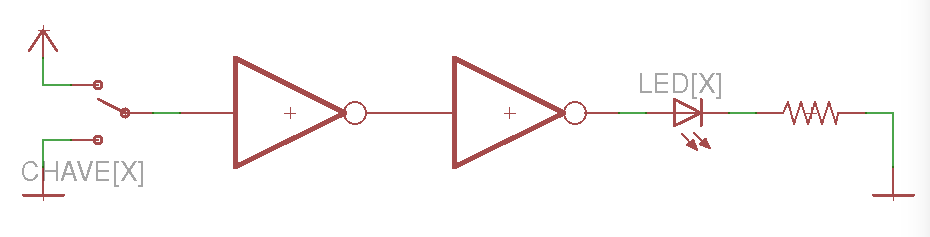
\includegraphics[width=1\textwidth]{desafio1_sch.png}
    \caption{Esquemático simplificado do desafio 1.}
    \label{fig:desafio1_sch}
\end{figure}

Abaixo, o código \emph{VHDL} da implementação.

\inputminted{vhdl}{Desafio1.vhd}


\subsection{Mapeamento das portas I/0}
\label{subsec:desafio1_map}

Abaixo, o mapeamento das entradas e saídas para o kit Nexys 2.

\inputminted{vhdl}{desafio2_pins.ucf}

\subsection{Simulação}

Para o teste do circuito, optou-se por simular o deslocamento de 1 bit na entrada, do menos significativo para o mais significativo, a cada 250ns.

Abaixo, o código \emph{VHDL} do Testbench.

\inputminted{vhdl}{tb_desafio1.vhd}

\begin{figure}[!h]
    \centering
    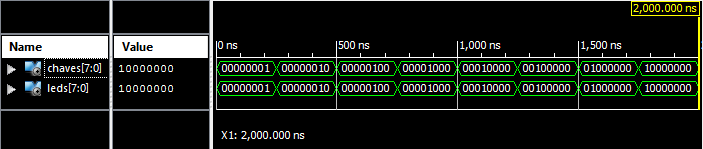
\includegraphics[width=1\textwidth]{tb_1.PNG}
    \caption{Resultado do testbench do desafio 1.}
    \label{fig:desafio1}
\end{figure}

\clearpage

\section{Desafio 2}

O segundo desafio propõe o acionamento dos LEDs a partir do nível lógico das chaves através das seguintes lógicas booleanas: o LSB da saída recebe o resultado da operação lógica AND entre o LSB e o MSB da entrada; o MSB da saída recebe o resultado da operação lógica OR entre o LSB e o MSB da entrada. Nestes casos, MSB se refere aos 4 bits mais significativos, e LSB aos 4 bits menos significativos.

\subsection{Implementação}

A implementação do sistema foi realizada através de 2 vetores (std\_logic\_vector) de 8 posições, onde cada posição da saída (LEDs) recebe o resultado da lógica descrita anteriormente.

A Figura~\ref{fig:desafio2_sch} exemplifica o circuito.

\begin{figure}[!h]
    \centering
    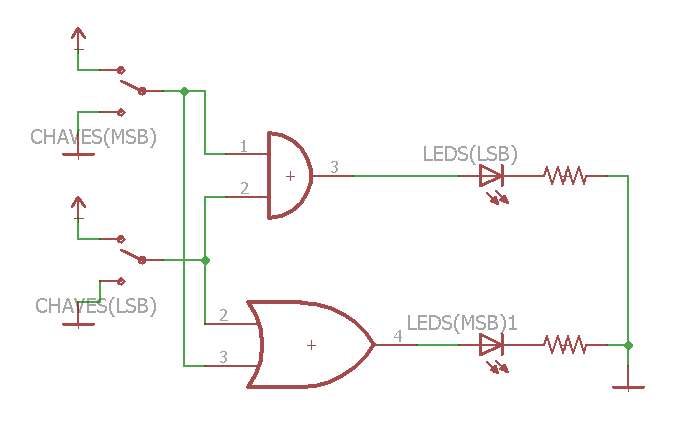
\includegraphics[width=0.7\textwidth]{desafio2_sch.png}
    \caption{Esquemático simplificado do desafio 2.}
    \label{fig:desafio2_sch}
\end{figure}


Abaixo, o código \emph{VHDL} da implementação.

\inputminted{vhdl}{Desafio2.vhd}

\subsection{Mapeamento das portas I/0}

O mapeamento das entradas e saídas é o mesmo do desafio 1 (tópico~\ref{subsec:desafio1_map}).

\subsection{Simulação}

Para o teste do circuito, optou-se por simular alguns valores na entrada e alterá-los a cada 250ns.

Abaixo, o código \emph{VHDL} do Testbench.

\inputminted{vhdl}{tb_desafio2.vhd}

\begin{figure}[!h]
    \centering
    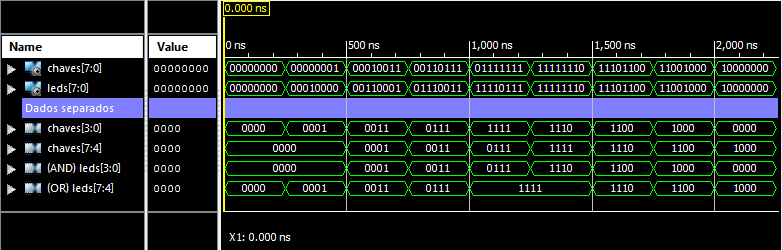
\includegraphics[width=1\textwidth]{tb_2.PNG}
    \caption{Resultado do testbench do desafio 2.}
    \label{fig:desafio2}
\end{figure}

\clearpage

\section{Desafio 3}

O terceiro desafio propõe a solução da tabela-verdade abaixo.

\begin{table}[htb]
\centering
\caption{Tabela-verdade do desafio 3.}
\label{true-table-3}
\begin{tabular}{llll|ll}
	\textbf{A} & \textbf{B} & \textbf{C} & \textbf{D} & \textbf{W} & \textbf{Z} \\ \hline
	0 & 0 & 0 & 0 & 1 & X \\
	0 & 0 & 0 & 1 & 0 & X \\
	0 & 0 & 1 & 0 & 1 & X \\
	0 & 0 & 1 & 1 & 0 & 1 \\
	0 & 1 & 0 & 0 & 1 & 1 \\
	0 & 1 & 0 & 1 & 1 & 0 \\
	0 & 1 & 1 & 0 & 1 & X \\
	0 & 1 & 1 & 1 & 1 & 1 \\
	1 & 0 & 0 & 0 & 1 & 0 \\
	1 & 0 & 0 & 1 & 0 & 0 \\
	1 & 0 & 1 & 0 & 1 & X \\
	1 & 0 & 1 & 1 & 0 & 0 \\
	1 & 1 & 0 & 0 & 0 & 0 \\
	1 & 1 & 0 & 1 & 0 & 0 \\
	1 & 1 & 1 & 0 & 0 & X \\
	1 & 1 & 1 & 1 & 0 & 0
\end{tabular}
\end{table}

\subsection{Implementação}
Através do método do Mapa de Karnaugh, obteve-se as seguintes expressões mínimas:

\begin{equation}
\centering
Z = (\bar{A} \cdot \bar{D}) + (\bar{A} \cdot C)
\end{equation}

\begin{equation}
\centering
W = (\bar{B} \cdot \bar{D}) + (\bar{A} \cdot B)
\end{equation}

A Figura~\ref{fig:desafio3_sch} exemplifica o circuito.
    
\clearpage

\begin{figure}[!h]
    \centering
    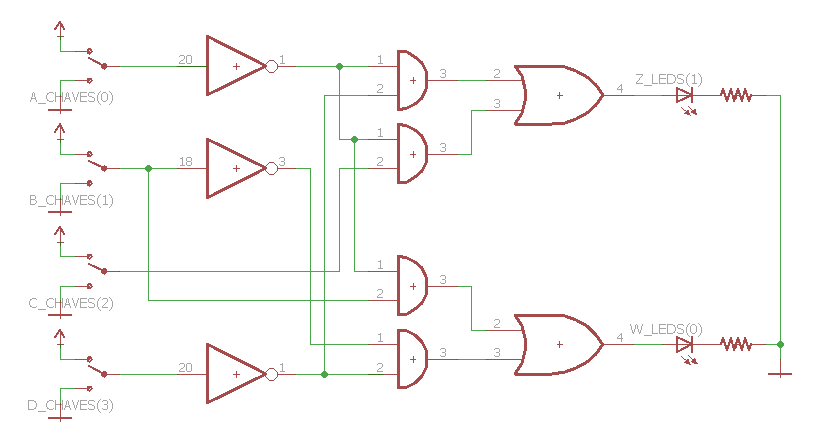
\includegraphics[width=1\textwidth]{desafio3_sch.png}
    \caption{Esquemático do desafio 3.}
    \label{fig:desafio3_sch}
\end{figure}

Abaixo, o código \emph{VHDL} da implementação.

\inputminted{vhdl}{Desafio3.vhd}

\subsection{Mapeamento das portas I/0}

Abaixo, o mapeamento das entradas e saídas para o kit Nexys 2.

\inputminted{vhdl}{desafio3_pins.ucf}

\subsection{Simulação}

Para o teste do circuito, optou-se por simular um incremento aritmético na entrada a cada 100ns. Desta forma, testou-se todos os valores (inclusive os não relevantes) entre 0x0 e 0xF.

Abaixo, o código \emph{VHDL} do Testbench.

\inputminted{vhdl}{tb_desafio3.vhd}

\begin{figure}[!h]
    \centering
    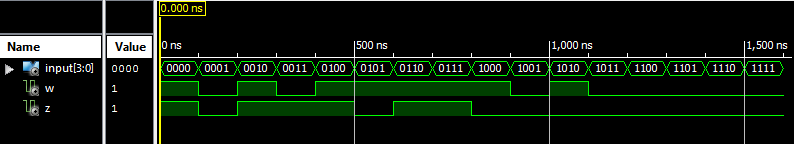
\includegraphics[width=1\textwidth]{tb_3.PNG}
    \caption{Resultado do testbench do desafio 3.}
    \label{fig:desafio3}
\end{figure}

A atribuição manual dos valores neste Testbench não é a mais elegante (referindo-se tecnicamente), porém foi a medida tomada após as dificuldades em implementar laços (\emph{for}) e operadores deslocamento (\emph{shift operators}), estes que serão retomados nos próximos laboratórios assim que surgirem oportunidades de implementação.


\end{document}
